
\section{Framework}
\label{sec:framework}

How our framework is structured

The first online multiplayer systems used peer-to-peer lockstep. With this method every client starts out in the same initial state and broadcasts every move made. This method works well for games that have clearly defined states and won’t be hindered by slow clients that have high latency~\cite{DOOMfaq}. 

To have better real-time support systems switched to a client/server model. With this model the state of the game is stored on the server and clients send in updates. This works well as latency is determined by the client to server connection (no slow client(s) halting the game). However, this was still too slow for real-time online games, which lead to the introduction of client-side prediction. Simply put client-side prediction allows the client to simulate its own version of the game (sending the results to the server) but the server can still step in and override the client's game state. This creates complexity in handling server overrides on clients smoothly (not just in code but also in animation and audio). There is a method for lag compensation, where the server runs in the past (simulation time), but we won’t go into this.

This gets very complicated, why have all the infrastructure? Why not just use a peer-to-peer (not lockstep) method? Two reasons, the first is that players could not join a game in progress. Second, the client can (and will) cheat, sending faulty position information to everyone in order to gain an advantage.

It would be nice if we could completely trust clients but we can’t. What if we could trust them a little? If we can trust clients a little we can use them as servers. If we can have a client as server we might be able to reduce latency by choosing the best client to act as the server.

What has not been mentioned in this discussion is fault tolerance. A client/server model has a single point of failure, the server. This can be very bothersome to players of the game that have invested a large amount of time into the game. 

Also having the single server model results in little fault tolerance. Not to mention the company has to construct many expensive servers so the clients can play.

Benefit of this solution:
Having a more fault tolerant system using a distributed server. 
Reducing latency by reducing by picking good servers
All online multiplayer systems are best effort. If we can create a system with the same responsiveness with fault tolerance then it is a success.

\begin{enumerate}
	\item Common mutiplayer model
	\begin{figure}
	\centering
	\begin{tabular}{c c}
		Peer-to-Peer & Client-Server \\
		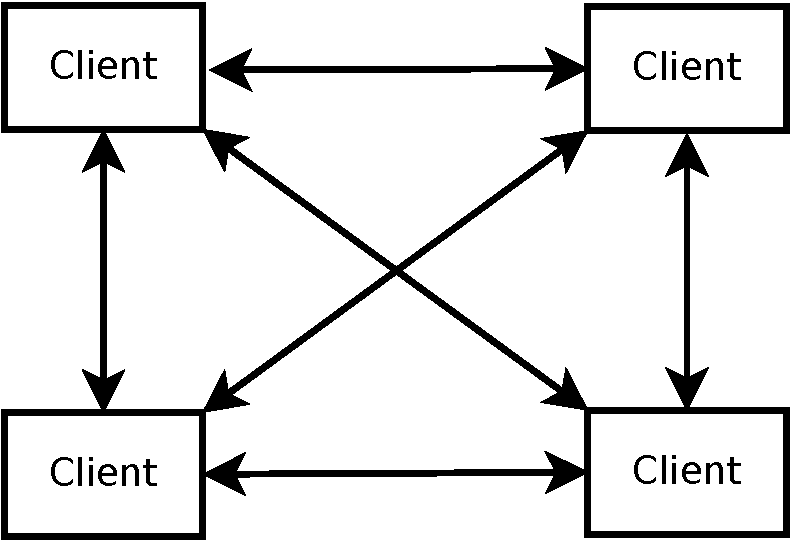
\includegraphics[width=0.48\linewidth]{../images/p2p-model-crop.pdf} &
		%trim=l b r t
		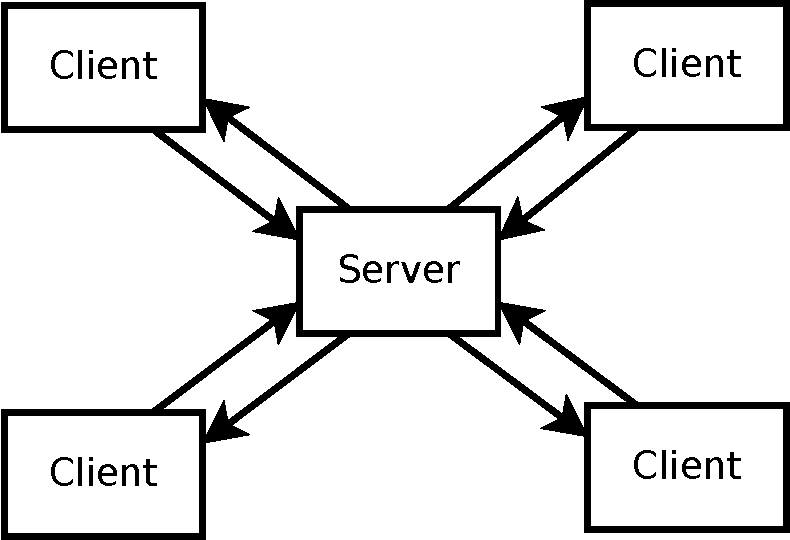
\includegraphics[width=0.48\linewidth]{../images/client-server-model-crop.pdf} \\
		(a) & (b)
	\end{tabular}

	\caption{\label{figure:p2p-vs-ClientServer} Two mutiplayer game networking models. The model on the left (a) is a peer-to-peer model where every client sends updates directly to ever other client in the game. The second model (b) is a client server model. In this model all of the clients send updates to the server and the server send updates out to the clients.}
	\end{figure}
	\begin{enumerate}
		\item latency minimization
		\item distributed state synchronization
		\item Avoiding cheating
	\end{enumerate}
	\item How Clients work
	\begin{enumerate}
		\item Client data
		\item Client messaging
	\end{enumerate}

	\item How the server works
	\begin{enumerate}
		\item Server data
		\item Server messaging
	\end{enumerate}
	\item The Game
	\begin{enumerate}
		\item Game data
		\item Game events/messaging
		\begin{enumerate}
			\item move
			\item fire
		\end{enumerate}
	\end{enumerate}
	\item Distributing the game
	\begin{enumerate}
		\item {Two server example}
		\item {Many server example}
		\begin{enumerate}
			\item The best serves can be choosen between two clients and most likely it will be the server on one of the two clients.
		\end{enumerate}
	\end{enumerate}
\end{enumerate}
\todo{Up this point we have really only solved fault tolerance. If we want to solve some scalability issue we will need to provide spatial segmenting of the Game world.}

